% 
% Permission is granted to copy, distribute and/or modify this document
% under the terms of the GNU Free Documentation License, Version 1.2
% or any later version published by the Free Software Foundation;
% with no Invariant Sections, no Front-Cover Texts, and no Back-Cover
% Texts.  A copy of the license is included in the section entitled "GNU
% Free Documentation License".

\documentclass[11pt]{article}

\usepackage{otfftw_Documentation}
\usepackage{Math_Notations}

\makeindex

\begin{document}

\thispagestyle{empty}

% 
% Permission is granted to copy, distribute and/or modify this document
% under the terms of the GNU Free Documentation License, Version 1.2
% or any later version published by the Free Software Foundation;
% with no Invariant Sections, no Front-Cover Texts, and no Back-Cover
% Texts.  A copy of the license is included in the section entitled "GNU
% Free Documentation License".
\vspace*{2cm}

\begin{center}
  {\huge \bf Documentation of the OpenTURNS-FFTW module}
  \input{GenericInformation.tex}
\end{center}



\newpage
%  
%  Permission is granted to copy, distribute and/or modify this document
%  under the terms of the GNU Free Documentation License, Version 1.2
%  or any later version published by the Free Software Foundation;
%  with no Invariant Sections, no Front-Cover Texts, and no Back-Cover
%  Texts.  A copy of the license is included in the section entitled "GNU
%  Free Documentation License".
\vspace{0.5in}
\begin{center}
\vspace{0.3in}
\emph{\fontshape{sc} Abstract}
\vspace{0.5in}
\end{center}

The purpose of this document is to present the OpenTURNS-FFTW module.

This document is organised according to the Open TURNS documentation :
\begin{itemize}
\item a \itshape{Reference Guide} which gives some theoretical basis,
\item a \itshape{Use cases Guide} which details scripts in python (the Textual Interface langage of Open TURNS) and helps the User to learn as quickly as possible the manipulation of the $otfftw$ module,
\item the \itshape{User Manual} which details the $otfftw$ objects and give the list of their methods,
\item the \itshape{Examples Guide} which provides at the moment only one example performed with the $otfftw$ module.
\end{itemize}


\tableofcontents
\newpage
% 
% Permission is granted to copy, distribute and/or modify this document
% under the terms of the GNU Free Documentation License, Version 1.2
% or any later version published by the Free Software Foundation;
% with no Invariant Sections, no Front-Cover Texts, and no Back-Cover
% Texts.  A copy of the license is included in the section entitled "GNU
% Free Documentation License".




%%%%%%%%%%%%%%%%%%%%%%%%%%%%%%%%%%%%%%%%%%%%%%%%%%%%%%%%%%%%%%%%%%%%%%%%%%%%%%%%%%%%%%%%%% 
\section{Reference Guide}

The OpenTURNS-FFTW library provides a bridge between the OpenTURNS library and the FFTW library, one of the most efficient implementation of the Fast Fourier Transform available to date. This library implements both the direct and inverse discrete Fourier transform.

More precisely, given a complex-valued sequence $(z_0,\dots,z_{n-1})$, its direct discrete Fourier transform $\Hat{z}=(\Check{z}_0,\dots,\Hat{z}_{n-1})$ reads:
$$
\Hat{z}_k = \sum_{j=0}^{n-1}z_j e^{-2i\pi\frac{jk}{n}}
$$
and its inverse discrete Fourier transform $\Check{z}=(\Check{z}_0,\dots,\Check{z}_{n-1})$ reads:
$$
\Check{z}_k = \frac{1}{n}\sum_{j=0}^{n-1}z_j e^{2i\pi\frac{jk}{n}}
$$

which gives the relation $z=\Check{\Hat{z}}$.

It is worth noting that the FFTW library does not include the $\frac{1}{n}$ normalization factor for the inverse transform. The FFTW library provides an $\mathcal{O}(n\log n)$ complexity implementation of such transforms even for prime $n$, but the best performance is achieved when $n$ is a power of 2.
\newpage
% 
% Permission is granted to copy, distribute and/or modify this document
% under the terms of the GNU Free Documentation License, Version 1.2
% or any later version published by the Free Software Foundation;
% with no Invariant Sections, no Front-Cover Texts, and no Back-Cover
% Texts.  A copy of the license is included in the section entitled "GNU
% Free Documentation License".




%%%%%%%%%%%%%%%%%%%%%%%%%%%%%%%%%%%%%%%%%%%%%%%%%%%%%%%%%%%%%%%%%%%%%%%%%%%%%%%%%%%%%%%%%% 
\section{Use Cases Guide}

This section presents the main functionalities of the module $otfftw$ in their context.



%%%%%%%%%%%%%%%%%%%%%%%%%%%%%%%%%%%%%%%%%%%%%%%%%%%%%%%%%%%%%%
\subsection{Which python modules to import ?}

In order to use the functionalities described in this documentation, it is necessary to import  : 
\begin{itemize}
   \item the $otfftw$ module which links the $openturns$ module.
\end{itemize}

Python  script for this use case :

\begin{lstlisting}
from otfftw import *
\end{lstlisting}

\subsection{Which python modules to import ?}

In order to use the functionalities described in this documentation, it is necessary to import  : 
\begin{itemize}
   \item the $openturns$ python module which gives access to the Open TURNS functionalities,
   \item the $otfftw$ module which links the $openturns$ module.
\end{itemize}

Python  script for this use case :

\begin{lstlisting}
# Load OpenTURNS to manipulate NumericalComplexCollection
from openturns import *
# Load the link between OT and FFTW
from otfftw import *
\end{lstlisting}

\subsection{UC: Using the FFTW algorithm to perform discrete Fourier transforms} \label{FFTWBasic}

With the $otfftw$ module, it is possible to perform both direct and inverse discrete Fourier transforms using the high-performance fftw library. To perform such transforms, the needed data are:

\requirements{
  \begin{description}
  \item[$\bullet$] a collection of complex values: {\itshape collection}
  \item[type:] NumericalComplexCollection
  \item[$\bullet$] the index of the first element to be transformed: {\itshape first}
  \item[type:] UnsignedInteger
 \item[$\bullet$] the size of the sub-sequence of values to be transformed: {\itshape size}
  \item[type:] UnsignedInteger
  \end{description}
}
{
  \begin{description}
  \item[$\bullet$] the transformed sequence : {\itshape transformedCollection},
  \item[type:] NumericalComplexCollection
  \end{description}
}
\espace

Python script for this use case:

\lstinputlisting[language=Python]{UC1_transform.py}

\subsection{UC: Using the FFTW algorithm to speed-up spectral process simulation} \label{FFTWSpectralProcess}

The fftw library is much more efficient than the FFT library provided by OpenTURNS. Knowing this point, OpenTURNS has been designed such that the TTF implementation can be plugged at run time for the most demanding algorithms. One of these algorithms is the simulation of SpectralProcess processes.

\requirements{
  \begin{description}
  \item[$\bullet$] a spectral normal process : {\itshape process}
  \item[type:] SpectralNormalProcess
  \item[$\bullet$] a sample size : {\itshape size}
  \item[type:] UnsignedInteger
  \end{description}
}
{
  \begin{description}
  \item[$\bullet$] a sample of size $size$ of the process : {\itshape sample},
  \item[type:] SampleProcess
  \end{description}
}
\espace

Python script for this use case:

\lstinputlisting[language=Python]{UC2_spectral.py}

\subsection{UC: Using the FFTW algorithm to speed-up spectral model estimation} \label{FFTWWelchFactory}

The same way the FFTW class can be used to speed-up the SpectralNormal class, it can be used to speed-up the WelchFactory class.

\requirements{
  \begin{description}
  \item[$\bullet$] a process sample : {\itshape sample}
  \item[type:] ProcessSample
  \item[$\bullet$] a Welch factory : {\itshape factory}
  \item[type:] WelchFactory
  \end{description}
}
{
  \begin{description}
  \item[$\bullet$] a spectral model : {\itshape spectralModel},
  \item[type:] UserDefinedSpectralModel
  \end{description}
}
\espace

Python script for this use case:

\lstinputlisting[language=Python]{UC3_Welch.py}


\newpage
% 
% Permission is granted to copy, distribute and/or modify this document
% under the terms of the GNU Free Documentation License, Version 1.2
% or any later version published by the Free Software Foundation;
% with no Invariant Sections, no Front-Cover Texts, and no Back-Cover
% Texts.  A copy of the license is included in the section entitled "GNU
% Free Documentation License".

%%%%%%%%%%%%%%%%%%%%%%%%%%%%%%%%%%%%%%%%%%%%%%%%%%%%%%%%%%%%%%%%%%%%%%%%%%%%%%%%%%%%%%%%%% 
\section{User Manual}

This section gives an exhaustive presentation of the objects and functions provided by the $otfftw$ module, in the alphabetic order.

\subsection{FFTW}


\begin{description}
\item[Usage :]  \strut
  \begin{description}
  \item $FFTW()$
  \end{description}
\item[Arguments :] None
\item[Value :]  a FFTW instance, it means an algorithm able to perform discrete Fourier transforms using the fftw library.
\item[Some methods :]  \strut

  \begin{description}

  \item $transform$
    \begin{description}
    \item[Usage :]  $transform(collection)$
    \item[Usage :]  $transform(collection, first, size)$
    \item[Arguments :]  \strut
      \begin{description}
      \item $collection$ : a NumericalComplexCollection of length $n$.
      \item $first$ : an integer, the index of the first element of $collection$ to be taken into account. We must have $first < n$.
      \item $size$ : an integer, the size of the sub-sequence of $collection$ to be transformed. We must have $first+size \leq n$.
      \end{description}
    \item[Value :] a NumericalComplexCollection, containing the direct discrete Fourier transform of the whole collection for the first usage and of the sub-sequence starting at position $first$ and of length $size$ for the second usage.
    \end{description}

  \item $inverseTransform$
    \begin{description}
    \item[Usage :]  $inverseTransform(collection)$
    \item[Usage :]  $inverseTransform(collection, first, size)$
    \item[Arguments :]  \strut
      \begin{description}
      \item $collection$ : a NumericalComplexCollection of length $n$.
      \item $first$ : an integer, the index of the first element of $collection$ to be taken into account. We must have $first < n$.
      \item $size$ : an integer, the size of the sub-sequence of $collection$ to be transformed. We must have $first+size \leq n$.
      \end{description}
    \item[Value :] a NumericalComplexCollection, containing the inverse discrete Fourier transform of the whole collection for the first usage and of the sub-sequence starting at position $first$ and of length $size$ for the second usage.
    \end{description}

  \end{description}

\end{description}
\newpage
% 
% Permission is granted to copy, distribute and/or modify this document
% under the terms of the GNU Free Documentation License, Version 1.2
% or any later version published by the Free Software Foundation;
% with no Invariant Sections, no Front-Cover Texts, and no Back-Cover
% Texts.  A copy of the license is included in the section entitled "GNU
% Free Documentation License".




%%%%%%%%%%%%%%%%%%%%%%%%%%%%%%%%%%%%%%%%%%%%%%%%%%%%%%%%%%%%%%%%%%%%%%%%%%%%%%%%%%%%%%%%%% 
\section{Examples Guide}

We present here an example of an uncertainty propagation study based on a representation of the uncertainty thanks to a normal process $X(t)$. We define the input normal process using a spectral model, then we sample this model and propagate it through a linear model $L(x)$. Then, we recover the spectral model of the output process $Y(t)$ based on the output sample. This study is FFT intensive, and all the computations will be done using the FFTW object.

The input process is of dimension 1, and based on a normalized Cauchy spectral model defined by a spectral density $S(f)$ such that:
$$
  \forall f\in\Rset,\quad S_X(f)=\frac{2}{1+(2\pi f)^2}
$$

The linear model $L(x)$ is simply a scaling transformation:
$$
  \forall x\in\Rset,\quad L(x)=\alpha x
$$

The theoretical output process $Y(t)$ is also normal, stationnary and its spectral density is given by:
$$
  \forall f\in\Rset,\quad S_Y(f)=\frac{2}{1+(2\pi f)^2}
$$

A graphical comparison between this theoretical spectral density and the reconstructed one is given on figure \ref{DSPComparison}.

\begin{figure}[h]
  \centering
  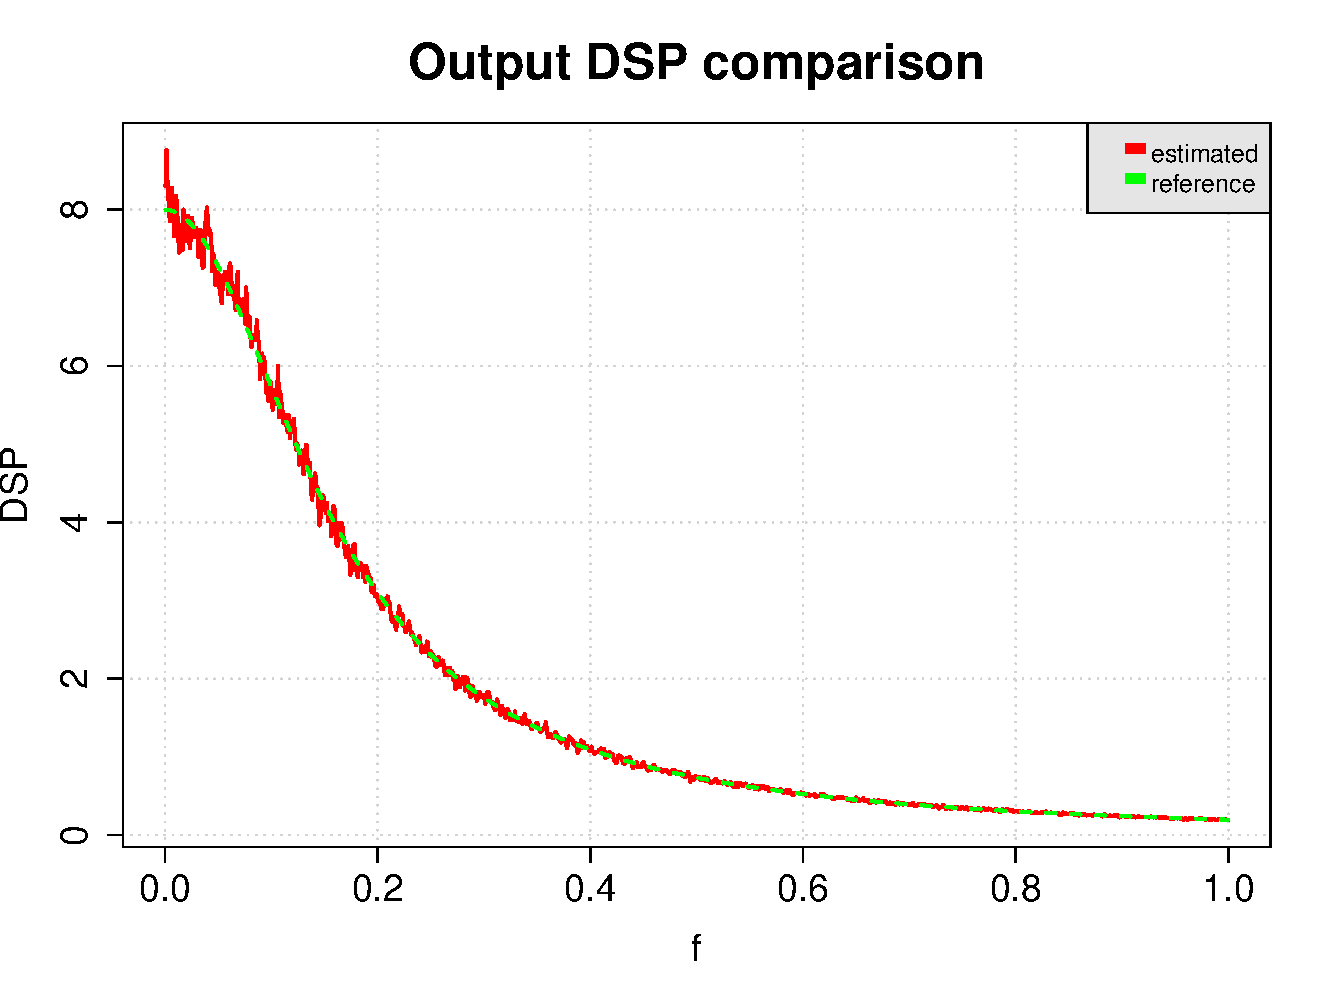
\includegraphics[width=\textwidth]{DSPComparison.pdf}
  \caption{Estimated spectral density (red) and theoretical one (green) of the output process}
  \label{DSPComparison}
\end{figure}

The speed-up with respect to the default OpenTURNS FFT algorithm is:
\begin{itemize}
\item a sampling time divided by a factor of 1.14
\item an estimation time divided by a factor of 2.31
\end{itemize}

on an Intel QuadCore Q9300 at 2.53GHz based laptop running Linux Mandriva 2010.2

\subsection{Python script}

\lstinputlisting[language=Python]{fftw_DSPEstimation.py}


\printindex
\end{document}
